\documentclass[notheorems]{beamer}

% Packages, common definitons, etc.
\usepackage[english]{babel}
\usepackage{graphicx}
\usepackage{tikz}

\usepackage{amsthm}
\setbeamertemplate{theorems}[numbered] % to number

\theoremstyle{definition}
\newtheorem{definition}{Definition}[section]
\newtheorem{example}[definition]{Example}
\theoremstyle{plain}
\newtheorem{theorem}[definition]{Theorem}
\newtheorem{lemma}[definition]{Lemma}
\newtheorem{corollary}[definition]{Corollary}
\def\Satzrefname{Satz}
\theoremstyle{remark}
\newtheorem*{remark}{Remark}


\newcommand{\N}{\mathbb{N}} % natural numbers
\newcommand{\Z}{\mathbb{Z}} % integers
\newcommand{\Q}{\mathbb{Q}} % rational numbers
\newcommand{\K}{\mathbb{K}} % field
\newcommand{\R}{\mathbb{R}} % reals
\newcommand{\C}{\mathbb{C}} % complex numbers
\newcommand{\1}{\mathds{1}} % indicator
\newcommand{\A}{\mathcal{A}}
\newcommand{\G}{\mathcal{G}}
\newcommand{\F}{\mathcal{F}}
\newcommand{\X}{\mathcal{X}}
\newcommand{\T}{\mathcal{T}}
\newcommand{\Zer}{\mathscr{Z}}
\newcommand{\m}{\mathfrak{m}}
\newcommand{\frakB}{\mathfrak{b}}
\newcommand{\M}{\mathscr{M}}
\newcommand{\Hol}{\mathcal{H}}


% End of packages, common definitions, etc.

\title{Energy Forms on Fractals}
\subtitle{The Case of the Sierpinksi Gasket}
\author{Youssef Hakiki \and Marcel Kleinfeller \and Paul Rahlf \and \\[3mm] {\small Supervisor: Uta Freiberg}}
\institute{ISem26 - Project D}
\date{\today}

\begin{document}
\begin{frame}
    \titlepage
\end{frame}

%\begin{frame}
%    \tableofcontents
%\end{frame}

\section{Graph approximations}
\begin{frame}{What is a fractal?}
    You know it, when you see it!

    \begin{columns}[c]
        \column{0.33\textwidth}
        \begin{figure}
            \centering
            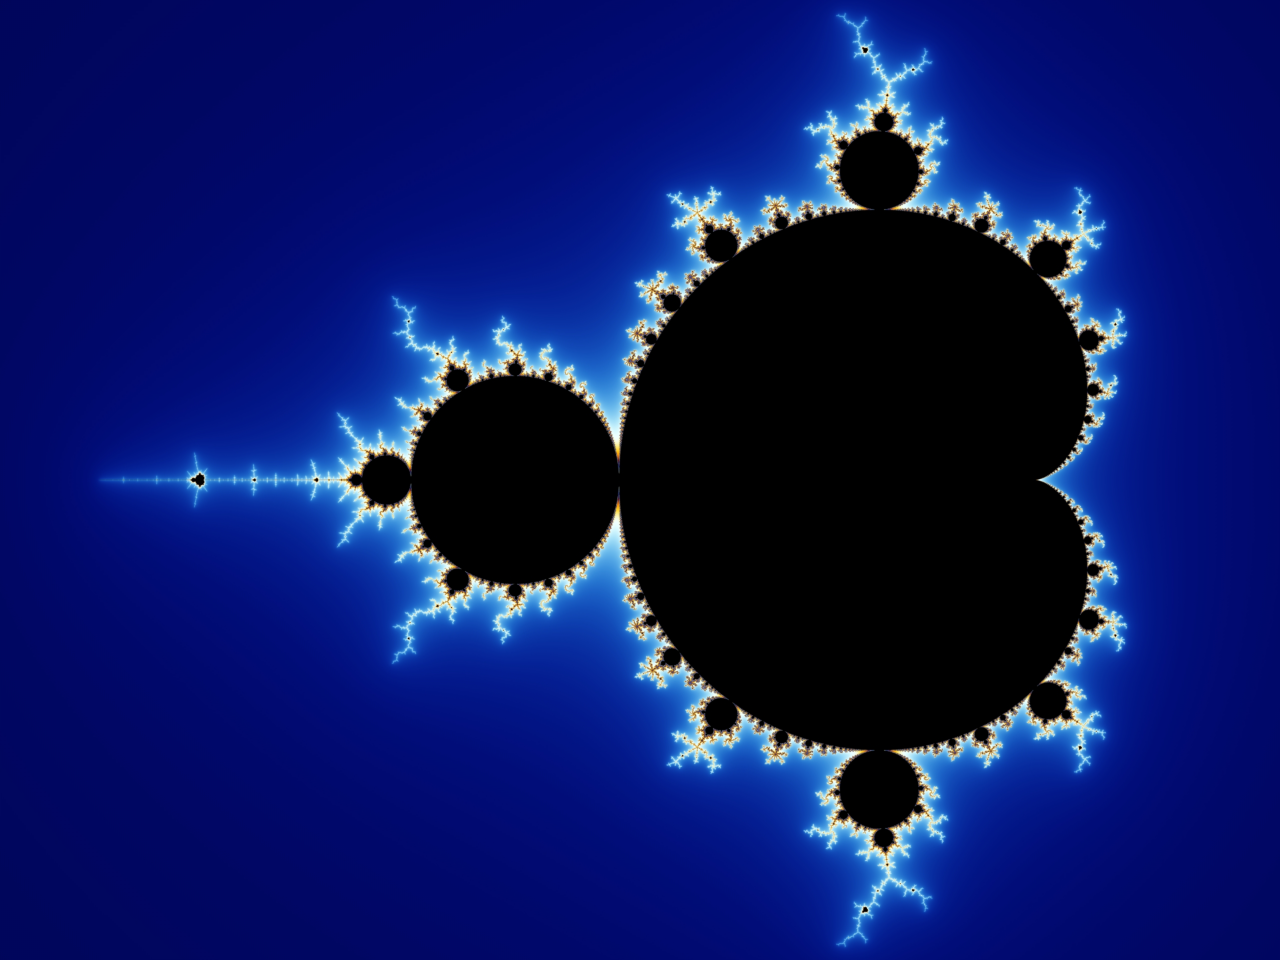
\includegraphics[height=5em]{images/mandelbrot.pdf}
            \caption{Mandelbrot set}
        \end{figure}
        \column{0.33\textwidth}
        \begin{figure}
            \centering
            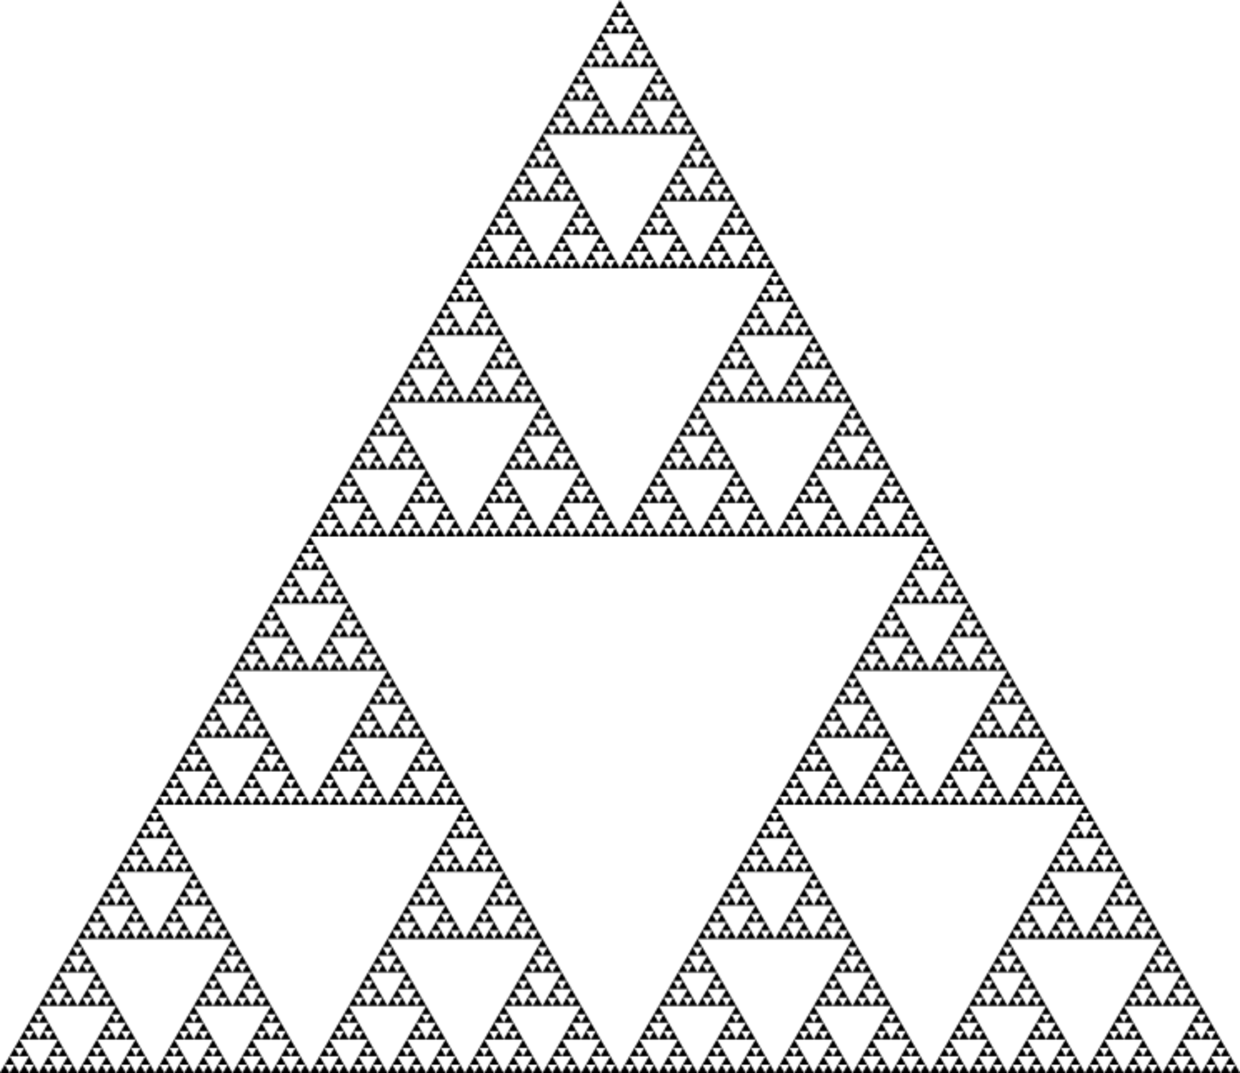
\includegraphics[height=5em]{images/sierpinksi.pdf}
            \caption{Sierpinksi gasket}
        \end{figure}
        \column{0.33\textwidth}
        \begin{figure}
            \centering
            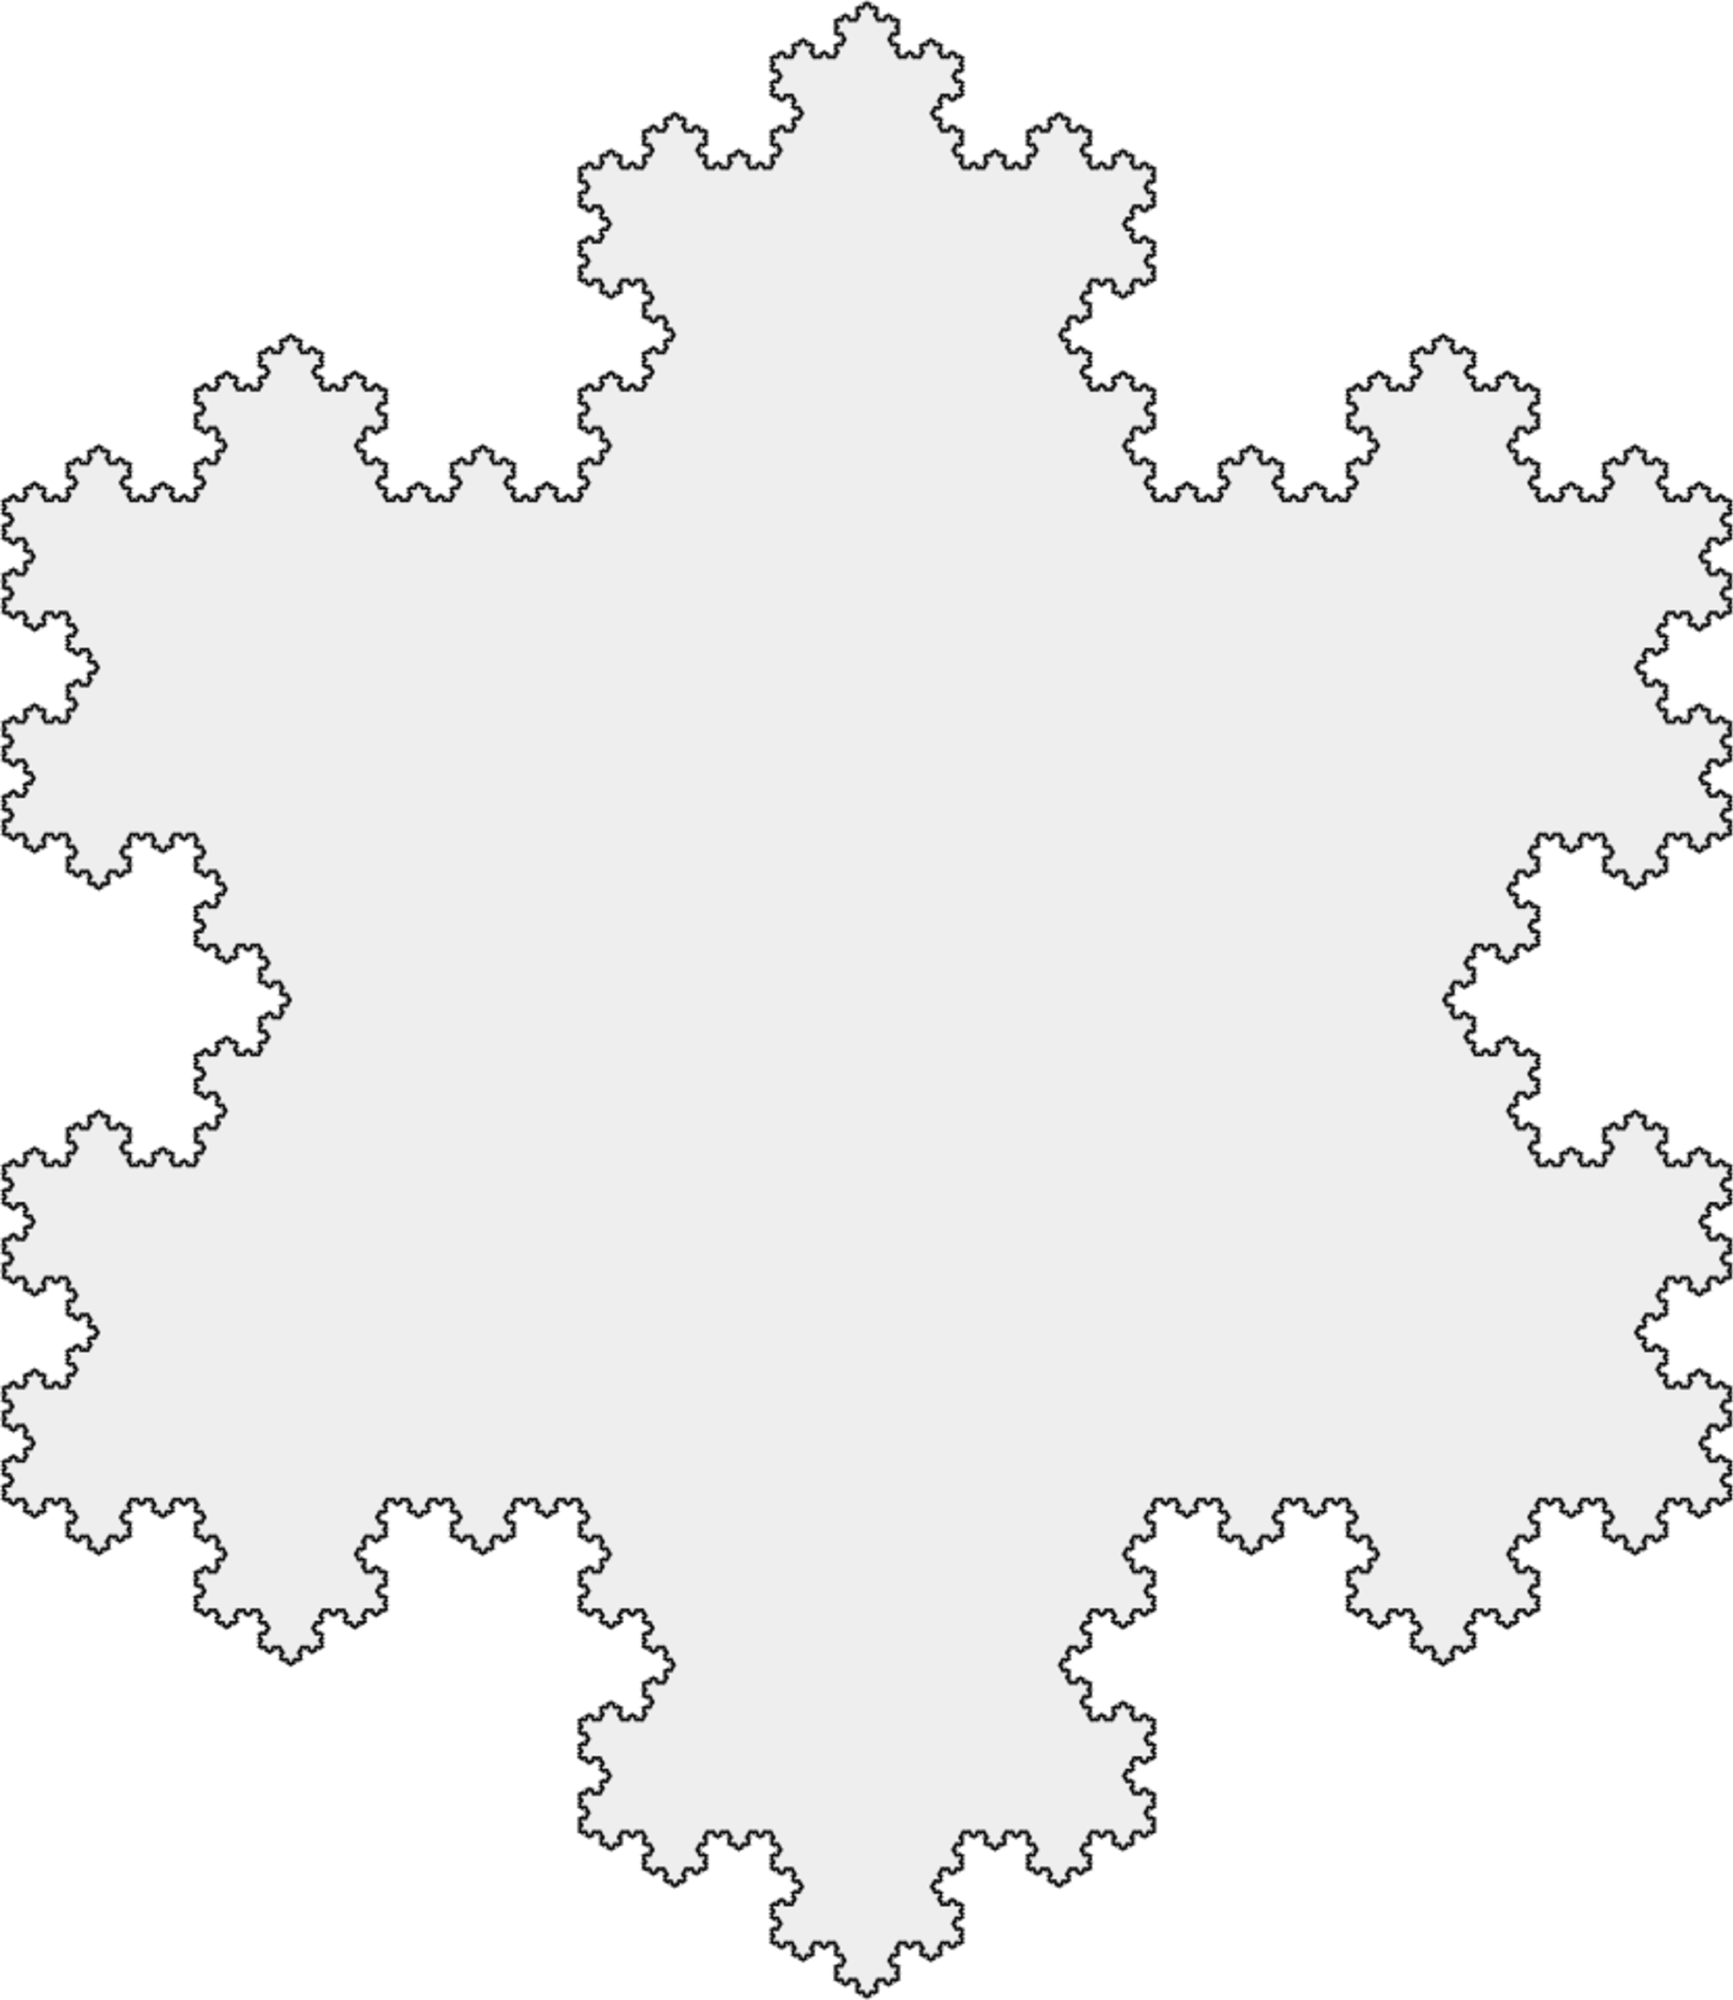
\includegraphics[height=5em]{images/snowflake.pdf}
            \caption{Koch snowflake}
        \end{figure}
    \end{columns}

    Common features: 
    \begin{itemize}
        \item self-similarity
        \item roughness
        \item infinitely detailed
        \item generate complex structure from very simple procedure (e.g. from iterated function systems)
    \end{itemize}
\end{frame}

\begin{frame}{Iterated function systems}
    \begin{definition}
        An \textit{iterated function system (IFS)} is a family \(F = \{ F_i: \R^d \to \R^d : 1 \leq i \leq N \ \} \) of contractions.
    \end{definition}

    \begin{theorem}[Hutchinson]
        There is a unique non-empty, compact set \(K \subset \R^d \) so that
        \[ K = F(K) := \bigcup_i F_i(K). \]
    \end{theorem}

    \begin{example}
        a) \textbf{Sierpinksi gasket:} Choose \(V_0 := \{q_0, q_1, q_2 \} \) as the verticies of a proper triangle. Then the contractions
        \[ F_i(x) := \frac{1}{2}(x - q_i) + q_i \]
        characterize the Sierpinksi gasket \(SG \subset \R^2 \).
    \end{example}
\end{frame}

\begin{frame}{Addressing points in IFS fractals}
    \addtocounter{definition}{-1}
    \begin{example}[Cont.]
        b) \textbf{Unit interval\footnote{Not a fractal, but a self-similar and a good prototype.}:} Choose \(V_0 := \{q_0 = 0, q_1 = 1 \} \). Then
        \[ F_i(x) := \frac{1}{2}(x - q_i) + q_i \]
        gives us the unit interval \(I \subset \R \).
    \end{example}

    Iteratively, define \(V_m := \bigcup_i F_i(V_{m-1}) \) and note that one can write
    \[ V_m = \bigcup_{| \omega | = m} F_\omega(V_0), \quad \text{where } F_\omega := F_{\omega_1} \circ \cdots \circ F_{\omega_m} \]
    and \(\omega \in \{1, \dots, N \}^m \) is a \textit{word} of length \(| \omega | = m \).

    So, every point \(x \in V_* := \bigcup_{m \geq 0} V_m \) can be written as \(x = F_\omega q_i \).  Every \(x \in V_m \setminus V_0 \) has exactly two addresses since \(F_0 q_1 = F_1 q_0 \), \(F_1 q_2 = F_2 q_1 \) and \(F_2 q_0 = F_0 q_2 \).
    Finally: Convince yourself, that \(K = \overline{V_*} \).
\end{frame}

\begin{frame}{Finite ramification and graph approximations}
    \begin{definition}
        \begin{enumerate}
            \item If \(\omega \) is a word of with length \(| \omega | = m \), we call \(F_\omega (K) \) a \textit{cell} of level \(m \).
            \item If two distinct cells of level \(m \) intersect in at most finitely many points, we say that \(K \) is \textit{finitely ramified}.
        \end{enumerate}
    \end{definition}

    In the case of \(K \in \{I, SG \} \), two distinct \(m \) level cells intersect in at most one point and the set of those \textit{junction points} is \(V_m \setminus V_0 \). We can thus define a relation on the set \(V_m \) through
    \[ x \sim_m y :\Leftrightarrow \text{there is a } \omega \text{ of length } | \omega | = m \text{ so that } x, y \in F_\omega K. \]

    Now, we can consider graphs \(\Gamma_m := (V_m, \sim_m) \).
\end{frame}

\begin{frame}{Graph approximations}
    \begin{example}[Graph approximations]
        \begin{enumerate}
            \item Unit interval:
        \begin{columns}[c]
            \column{0.33\textwidth}
            \begin{figure}
                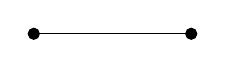
\begin{tikzpicture}[scale=2]
                    \draw (0,0) -- (1,0);
                    \filldraw [black] (0,0) circle (1pt);
                    \filldraw [black] (1,0) circle (1pt);
                \end{tikzpicture}\\
                \centering
                \(\Gamma_0 \)
            \end{figure}
            \column{0.33\textwidth}
            \begin{figure}
                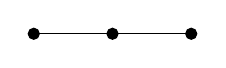
\begin{tikzpicture}[scale=2]
                    \draw (0,0) -- (1,0);
                    \filldraw [black] (0,0) circle (1pt);
                    \filldraw [black] (1,0) circle (1pt);
                    \filldraw [black] (0.5,0) circle (1pt);
                \end{tikzpicture}\\
                \centering
                \(\Gamma_1 \)
            \end{figure}
            \column{0.33\textwidth}
            \begin{figure}
                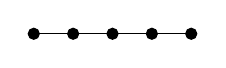
\begin{tikzpicture}[scale=2]
                    \draw (0,0) -- (1,0);
                    \filldraw [black] (0,0) circle (1pt);
                    \filldraw [black] (1,0) circle (1pt);
                    \filldraw [black] (0.5,0) circle (1pt);
                    \filldraw [black] (0.25,0) circle (1pt);
                    \filldraw [black] (0.75,0) circle (1pt);
                \end{tikzpicture}\\
                \centering
                \(\Gamma_2 \)
            \end{figure}
        \end{columns}
        \item Sierpinksi gasket:
        \begin{columns}[c]
            \column{0.33\textwidth}
            \begin{figure}
                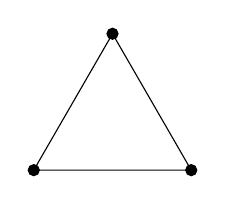
\begin{tikzpicture}[scale=2]
                    \draw (0,0) -- (1,0) -- (0.5,0.866) -- (0,0);
                    \filldraw [black] (0,0) circle (1pt);
                    \filldraw [black] (1,0) circle (1pt);
                    \filldraw [black] (0.5,0.866) circle (1pt);
                \end{tikzpicture}\\
                \centering
                \(\Gamma_0 \)
            \end{figure}
            \column{0.33\textwidth}
            \begin{figure}
                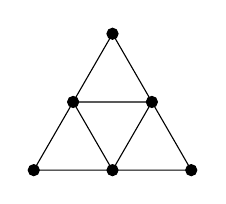
\begin{tikzpicture}[scale=2]
                    \draw (0,0) -- (1,0) -- (0.5,0.866) -- (0,0);
                    \draw (0.5,0) -- (0.25,0.433) -- (0.75,0.433) -- (0.5,0);
                    \filldraw [black] (0,0) circle (1pt);
                    \filldraw [black] (1,0) circle (1pt);
                    \filldraw [black] (0.5,0.866) circle (1pt);
                    \filldraw [black] (0.5,0) circle (1pt);
                    \filldraw [black] (0.25,0.433) circle (1pt);
                    \filldraw [black] (0.75,0.433) circle (1pt);
                \end{tikzpicture}\\
                \centering
                \(\Gamma_1 \)
            \end{figure}
            \column{0.33\textwidth}
            \begin{figure}
                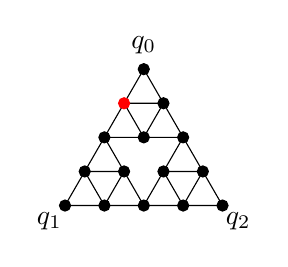
\begin{tikzpicture}[scale=2]
                    \draw (0,0) -- (1,0) -- (0.5,0.866) -- (0,0);
                    \draw (0.5,0) -- (0.25,0.433) -- (0.75,0.433) -- (0.5,0);
                    \draw (0.5,0.433) -- (0.375,0.6495) -- (0.625,0.6495) -- (0.5,0.433);
                    \draw (0.25,0) -- (0.125,0.2165) -- (0.375,0.2165) -- (0.25,0);
                    \draw (0.75,0) -- (0.625,0.2165) -- (0.875,0.2165) -- (0.75,0);
                    \filldraw [black] (0,0) circle (1pt);
                    \node[yshift=-2mm, xshift=-2mm] at (0,0) {\(q_1\)};
                    \filldraw [black] (1,0) circle (1pt);
                    \node[yshift=-2mm, xshift=2mm] at (1,0) {\(q_2\)};
                    \filldraw [black] (0.5,0.866) circle (1pt);
                    \node[yshift=3mm, xshift=0mm] at (0.5,0.866) {\(q_0\)};
                    \filldraw [black] (0.5,0) circle (1pt);
                    \filldraw [black] (0.25,0.433) circle (1pt);
                    \filldraw [black] (0.75,0.433) circle (1pt);
                    \filldraw [black] (0.25,0) circle (1pt);
                    \filldraw [black] (0.75,0) circle (1pt);
                    \filldraw [black] (0.125,0.2165) circle (1pt);
                    \filldraw [black] (0.375,0.2165) circle (1pt);
                    \filldraw [black] (0.625,0.2165) circle (1pt);
                    \filldraw [black] (0.875,0.2165) circle (1pt);
                    \filldraw [black] (0.5, 0.433) circle (1pt);
                    \filldraw [red] (0.375,0.6495) circle (1pt);
                    \filldraw [black] (0.625,0.6495) circle (1pt);
                \end{tikzpicture}\\
                \centering
                \(\Gamma_2 \)
            \end{figure}
        \end{columns}
    \end{enumerate}
    \end{example}
    The red vertex is in \(V_2 \) and is addressed via \(x = F_{(0, 1)}q_0 = F_{(0,0)}q_1 \).
\end{frame}

\begin{frame}{Self-similar measures}
    \textbf{Want:} A measure \(\mu \) on \((K, \Sigma) \) which plays nicely with the self-similar structure of \(K \).

    Therefore, let \(\Sigma \) be the \(\sigma \)-field generated by all the cells of \(K \), set
    \[ \mu(F_\omega SG) := \left(\frac{1}{3} \right)^{|\omega |} \]
    and extend it to \(\Sigma \) by Carathéodory.

    In the case of the unit interval, it is easy to see that \( \mu(F_\omega I) := \left( \frac{1}{2} \right)^{|\omega |} \) extends to the Lebesgue measure.

    \begin{definition}
        We call the measure \(\mu \) \textit{self-similar} since
        \[ \mu(A) = \sum_i \mu_i \mu(F_i^{-1} A) \text{ for all } A \in \Sigma \]
        for some positive weights with \(\sum_i \mu_i = 1 \).
    \end{definition}
\end{frame}

\begin{frame}{Integration}
    We have canoncial measures on \(K \in \{I, SG \} \), so we can integrate measurable functions \(f: (K, \Sigma) \to (\R, \mathcal{B}) \).
    \begin{lemma}
        For \(f: K \to \R \) continuous, we obtain the usual Riemann integral via
        \[ \int_K f d\mu := \lim_{m \to \infty} \sum_{|\omega | = m} f(x_\omega) \mu(F_\omega K) \]
        for some \(x_\omega \in F_\omega K \).

        This can\footnote{for measure with standard weights} also be written with a measure \(\nu_m: V_m \to \R_+ \) as
        \begin{align*}
            \int_K f d\mu &= \lim_{m \to \infty} \frac{1}{3} \sum_{i=0}^2 \sum_{| \omega | = m} f(F_\omega q_i) \mu(F_\omega K)
            = \lim_{m\to \infty} \int_{V_m} f(x) d\nu_m(x) \\
            &\overset{\text{SG}}= 3^{-m} \left(\frac{2}{3} \sum_{x\in V_m \setminus V_0} f(x) + \frac{1}{3} \sum_{x \in V_0} f(x) \right).
        \end{align*}
    \end{lemma}
\end{frame}

\begin{frame}{Dirichlet principle}
    \textbf{Motivation:} The Dirichlet principle states: Solving the Poisson equation
    \[ \begin{cases}
            -\Delta u = f &\text{in } U,\\
            u = g &\text{on } \partial U
        \end{cases} \]
    is equivalent to minimization of the energy functional
    \[ E[v] = \frac{1}{2} \textcolor{red}{\int_U \| \nabla v(x) \|^2 dx} - \int_U f(x)v(x) dx \]
    on a suitable function space.

    \textbf{Aim:} Define something like the \textcolor{red}{red} energy via graph approximations for (continuous / measurable) functions \(f: K \to \R \).

    Use the unit interval \(I = [0, 1] \) as our model case.
\end{frame}

\begin{frame}{Graph energies for unit interval}
    \textbf{Note that:}
    \begin{align*}
        \int_U \| u'(x) \|^2 dx &\overset{\text{MVT}}= \lim_{m \to \infty} \sum_{k=1}^{2^m} 2^{-m} \left( \frac{u(k2^{-m}) - u((k-1)2^{-m})}{2^{-m}} \right)^2 \\
        &= \lim_{m \to \infty} 2^m \sum_{x \sim_m y} [ u(x) - u(y) ]^2 \\
        &=: \lim_{m \to \infty} r^{-m} E_m(u) =: \lim_{m\to\infty} \mathcal{E}_m (u)
    \end{align*}

    \textbf{Alternative way:} One can show via harmonic extensions that
    \[ E_{m+1}(u) \geq E_{m+1}(\tilde{u}) = r \cdot E_m(u) \]
    and thus
    \[ \mathcal{E}_{m+1}(u) = r^{-(m+1)} E_{m+1}(u) \geq r^{-m} E_m(u) = \mathcal{E}_m(u) \]
\end{frame}
\section{Graph Energies}
\begin{frame}{Graph Energies}
\begin{itemize}
    \item The graph energy, on a connected finite graph G, is defined as
    \begin{equation}
        E_G(u):=\underset{x \thicksim y}{\sum}\left(u(x)-u(y)\right)^2
    \end{equation}
    
    \item It is a quadratic form in $u$ associated to the following bilinear form
    \begin{equation}
        E_G(u,v):= \underset{x\thicksim y}{\sum}\left(u(x)-u(y)\right)\left(v(x)-v(y)\right)
    \end{equation}
\end{itemize}

Let's denote by $G:=(V,E)$, where
$$
\left\{
\begin{array}{rcl}
   V= &\text{ \,set of vertices}  \\
   E= &\text{ set of edges}.
\end{array}\right.
$$
\end{frame}
\begin{frame}{Markov Property (Compatibility with  with normal contraction)}
\begin{itemize}
    \item If $u:V \rightarrow \mathbb{R}_+$, we denote by $[u]=\min\{1,u\vee 0\}$. Then the energy $E_G(\cdot)$ satisfies the so called \textbf{Markov Property}, which is
    \begin{equation}
    E_G([u])\leq E_G(u).
    \end{equation}
    \item Let $G':=(V',E')$ such that $G\subseteq G'$ is a sub-graph. For $u:V \rightarrow \mathbb{R}_+$ given, $\,\,\exists$ $\tilde{u}: V' \rightarrow \mathbb{R}$ such that $\tilde{u}\lvert_V=u$ and that 
    $$
\underset{u'\lvert_V=u}{\inf}E_{G'}(u')=E_{G'}(\tilde{u})
    $$
\item $\tilde{u}$ is called the \textbf{harmonic extension}

\item For all examples of interest to us ($I$ and $SG$ included) we have
\begin{equation}
    E_{G'}(\tilde{u})=r\,E_G(u) \quad \text{ for all } u: V \rightarrow \mathbb{R}.
\end{equation}
for some $r\in (0.1)$. This called the \textbf{renormalization equation}.
\end{itemize}
\end{frame}

\begin{frame}
Therefore we have
\begin{equation}
    \frac{1}{r}\,E_{G'}(u')\geq E_G(u).
\end{equation}
This means that energy increase with \textbf{general extension}, except in the case of harmonic extension where the energy is \textbf{constant}.
\begin{example}
    Let's consider $K=SG$ and suppose $u(\cdot)$ is defined on $V_0$ by 
$$
\left\{
\begin{array}{rcl}
   u(q_0)=a  \\
   u(q_1)=b&.\\
   u(q_0)=c&
\end{array}\right.
$$
Then 

\begin{align*}
    E_1(\tilde{u})&=(a-z)^2+(b-z)^2+(b-x)^2+(c-x)^2+\\
    &+(a-y)^2+(c-y)^2+ (x-y)^2+(z-y)^2+(x-z)^2.
\end{align*}
is to be minimized.
\end{example}
\end{frame}
\begin{frame}
\begin{figure}
\centering
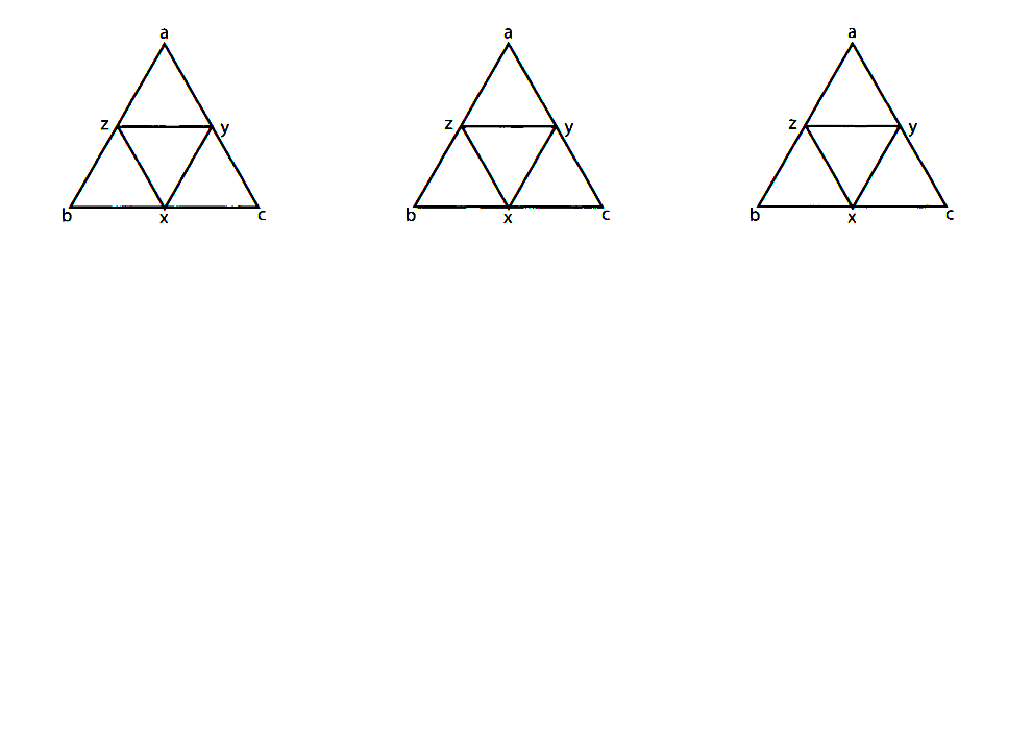
\includegraphics[height=5em]{images/harmonic extension order 1.pdf}
\caption{harmonic extension on $V_1$}
\end{figure}

\begin{itemize}
\item By calculating partial derivatives on x,y and z, we obtain 
\begin{align}\label{1st harm extension}
    %\begin{aligned}
    \left\{ \begin{array}{rcl}
        u(F_0q_1)=u(F_1q_0)=x:=& {\color{red} \frac{1}{5}}a+{\color{blue} \frac{2}{5}}b+{\color{blue} \frac{2}{5}}c \\
        \\
        u(F_0q_2)=u(F_2q_0)=y:=& {\color{blue} \frac{2}{5}}a+{\color{red} \frac{1}{5}}b+{\color{blue} \frac{2}{5}}c \\
        \\
        u(F_1q_2)=u(F_2q_1)=z:=& {\color{blue} \frac{2}{5}}a+{\color{blue} \frac{2}{5}}b+{\color{red} \frac{1}{5}}c \\
    \end{array}\right.
    %\end{aligned}
\end{align}

\item In the particular \textbf{symmetric} case, i.e. when $a=1$ and $b=c=0$, we obtain $x=1/5$ and $y=z=2/5$. 
\end{itemize}
\end{frame}
\begin{frame}
\begin{itemize}
    \item Using \eqref{1st harm extension}, we can show easily that 
    \begin{align}
        E_1(\tilde{u})=rE_0(u),
    \end{align}
    where $r=3/5$, so the \textbf{renormalized energy} is given by:
    $$
    \mathcal{E}_{1}(\tilde{u}):=r^{-1}E_1(\tilde{u})=E_0(u).
    $$
\item $\tilde{u}$ is the \textbf{harmonic extension} from $V_1$ to $V_2$.

\item The same idea could be done, for $u:V_m\rightarrow \mathbb{R}$ given, to obtain the \textbf{harmonic extension} form $V_m$ to $V_{m+1}$ such that:
\begin{align}
    \left\{ \begin{array}{cc}
        &E_{m+1}(\tilde{u})=rE_{m}(u)   \\
        &\mathcal{E}_{m+1}(\tilde{u})=r^{-1}E_{m}(u) 
    \end{array}\right.
\end{align}
\end{itemize}    
\end{frame}
\begin{frame}
    \begin{itemize}
        \item If $u:V_m\rightarrow \mathbb{R}$ is given and $u':V_{m+1}\rightarrow \mathbb{R}$ to be any arbitrary extension, then 
        \begin{align}
        E_{m+1}(u')=\underset{|\omega|=m}{\sum}E_1(u'\circ F_{\omega})    
        \end{align}
        and 
        \begin{align}
        E_{m+1}(u')=\underset{i=0,1,2}{\sum}E_m(u'\circ F_{i})    
        \end{align}
        
        \item The renormalized energy 
        $$
        \mathcal{E}_{m}(u)=(3/5)^{-m}\,E_{m}(u).,
        $$
        is constant under the harmonic extension. Moreover, it's a nondecreasing sequence for any extension. i.e.
        \begin{align}
            \mathcal{E}_{0}(u)\leq \mathcal{E}_{1}(u)\leq \ldots.
        \end{align}
    \end{itemize}
\end{frame}
\begin{frame}{Summary}
    TO summarize: Let $u$ be a function on $V_m$, then the harmonic extension $\tilde{u}$ to $V_{m+1}$ may be characterized in three ways:
    \vspace{0.25cm}
\begin{itemize}
    \item[(i)] it minimizes $\mathcal{E}_{m+1}(\tilde{u})$ at the value $\mathcal{E}_m(u)$;
    \item[(ii)] at each new point $x \in V_{m+1} \backslash V_m, \tilde{u}(x)$ is \textbf{the average of the values at the four neighboring points in} $V_{m+1}$; i.e. 
    $$
\tilde{u}(x)=\dfrac{1}{4}\underset{\substack{y \in V_{m+1} \\ y \underset{m+1}{\thicksim} x}}{\sum}\tilde{u}(y)
    $$
    \item[(iii)] it satisfies the " $\frac{1}{5}-\frac{2}{5}$ rule" at the new points in $V_{m+1} \backslash V_m$. 
\end{itemize}
\end{frame}
\section{Energy}
\begin{frame}{Energy}
\begin{itemize}
\item Since, for any function $u$ on $V_*$, the sequence of energies $\mathcal{E}_{m}(u)$ is nondecreasing. It make sense to define 
$$
\mathcal{E}(u):=\lim_{m\rightarrow +\infty}\mathcal{E}_{m}(u).
$$

\item Moreover 
\begin{align}\label{when energy vanish}
\mathcal{E}(u)=0 \quad \Leftrightarrow \quad u=const, 
\end{align}
and 
\begin{align}\label{dom energy}
\operatorname{dom}(\mathcal{E})=\left\{ u:V_*\rightarrow \mathbb{R}\,:\,\, \mathcal{E}(u)<\infty \right\}.
\end{align}
\end{itemize}
\end{frame}
\begin{frame}{Consequences}
\begin{itemize}
\item Let $u:V_*\rightarrow \mathbb{R}$ such that $\mathcal{E}(u)<\infty$. Therefore
\begin{align}
\lvert u(x)-u(y)\rvert\leq r^{m/2}\,\mathcal{E}^{1/2}(u)\quad \text{for all } x\underset{m}{\thicksim} y\in V_m.
\end{align}

\vspace{0.25cm}
\item From the geometry of $K$ (either I or SG) it can be seen that if $x,y\in V_*$ belong to the \textbf{same} or \textbf{adjacent} $m$-cell, with some technical calculation, we obtain 
\begin{align}\label{mod-cont}
\lvert u(x)-u(y)\rvert  \leq \frac{r^{m/2}}{1-r^{1/2}}\, \mathcal{E}^{1/2}(u).
\end{align}

\item When $K=I$ is the \textbf{interval}, \eqref{mod-cont} ensures that $u$ is $1/2$-Hölder continuous. Precisely; since $r=1/2$, if $x,y$ are such that $|x-y|\leq 1/2^{m}$ then $x$ and $y$ belongs to the same or adjacent $m$-cell. Hence \eqref{mod-cont} ensures that
\begin{equation}
    |u(x)-u(y)|\leq M |x-y|^{1/2}.
\end{equation}
%\item Moreover, for $x_m,x_{m+1},\ldots,x_{m+k}$ such that 
%$$
%\left\{\begin{array}{cc}
%& x_{m+j}\in V_{m+j}  \\
%& x_{m+j}\underset{m+j+1}{\thicksim} x_{m+j+1}
%\end{array}\right.,
%$$
%then 
%\begin{align}
%\lvert u(x_m)-u(x_{m+k})\rvert & \leq r^{m/2}\left(1+r^{1/2}+\ldots+r^{k/2}\right)\,\mathcal{E}^{1/2}(u)\nonumber \\
%& \leq \frac{r^{m/2}}{1-r^{1/2}}\, \mathcal{E}^{1/2}(u).
%\end{align}
\end{itemize} 
\end{frame}

\begin{frame}
\begin{itemize}
\item When $K=SG$, the $1/2$-Hölder continuity can be obtained in \textbf{another metric}, called the \textbf{resistance metric}, which we denote by $R(\cdot,\cdot)$. Hence if $u\in \operatorname{dom}(\mathcal{E})$ then for all $m\geq 1$
\begin{equation}
    \lvert u(x)-u(y)\rvert \leq M\cdot R(x,y)^{1/2}, 
\end{equation}
for all $x,y \in K$ such that $R(x,y)\leq r^{m}$.

\item Moreover, this resistance metric $R(\cdot,\cdot)$ is equivalent to the Euclidean metric with some exponent $0<\beta<1$, i.e. 
\begin{equation}
R(x,y)\thicksim \lVert x-y \rVert^{\beta} \quad \text{ for } \quad \beta=\log \frac{5}{3}/\log 2. 
\end{equation}
\end{itemize}
\end{frame}

\begin{frame}{Hilbert space property}
\begin{theorem}
    $dom(\mathcal{E})/constants$ forms a Hilbert space with the inner product given by 
    \begin{equation}\label{inner prod}
        (u,v)_{\mathcal{E}}:=\mathcal{E}(u,v):=\lim_{m\rightarrow \infty}\mathcal{E}_m(u,v) \quad \text{ for all } u,v \in \operatorname{dom}(\mathcal{E})
    \end{equation}
\end{theorem}
\end{frame}

\begin{frame}{Self-Similarity of the energy}
\begin{theorem}
If $u \in \operatorname{dom}(\mathcal{E})$ then $u \circ F_i \in \operatorname{dom}(\mathcal{E})$ for all $i$, and
\begin{align}\label{self-sim energy}
    \mathcal{E}(u)=\sum_i r^{-1} \mathcal{E}\left(u \circ F_i\right)
\end{align}
\end{theorem}
This self-similarity of the energy follows from the following fact
$$
\mathcal{E}_{m+1}(u)=\sum_{i=0}^{2} r^{-1} \mathcal{E}_m\left(u \circ F_i\right).
$$
Moreover, for any partition $\mathcal{P}$, using the subdivision:
\begin{equation}
    K=\underset{\omega \in \mathcal{P}}{\bigcup}F_{\omega}K,
\end{equation}
and replacing $r^{-1}$ by $r^{-|\omega|}$, we obtain
\begin{align}\label{self-sim energy}
    \mathcal{E}(u)=\sum_{\omega\in \mathcal{P}} r^{-|\omega|} \mathcal{E}\left(u \circ F_{\omega}\right).
\end{align}
\end{frame}
\begin{comment}
\begin{frame}{Self-Similar measure}
\begin{itemize}
    \item The previous self-similarity equation suggest the existence of a measure $\nu_u$ defined through energies. More precisely, we have
    $$
    \nu_u\left(F_{\omega} K\right):=r^{-|\omega|} \mathcal{E}\left(u \circ F_{\omega}\right).
    $$
    \item Equivalently, we can check that 
    $$
    \nu_{u}(F_{\omega}K)=\lim_{m\rightarrow \infty}r^{-m}\underset{x \underset{m}{\thicksim} y\,\,:\,\,x,y\in F_{\omega}K}{\sum}\left(u(x)-u(y)\right)^{2}.
    $$
    \item It can be shown that, for all $u\in \operatorname{dom} \mathcal{E}$ we have 
    $$
    \nu_{u}\left(F_{\omega}K\right)\leq r^{|\omega|}\mathcal{E}(u)\quad \text{ for all } \omega \in \mathcal{P} .
    $$
\end{itemize}
\end{frame}

\end{comment}
\begin{frame}{Markov property/Compatibility with normal contraction}
    \begin{itemize}
    \item The {Markov property/Compatibility with normal contraction} holds for all $u\in \operatorname{dom}(\mathcal{E})$, i.e.
    $$
    \mathcal{E}([u])\leq \mathcal{E}(u), 
    $$
    where $[u]=min\{1, u\vee 0\}$.
    \end{itemize}
\end{frame}

% ============================================================
% §1.5 Electric Network Interpretation
% ============================================================

\section{Electric Network Interpretation}

\begin{frame}{Electric Network Interpretation}
    % \textbf{Terminology:}
    \begin{description}
        \item[Network] Nodes (vertices) $V$ and conductors (edges) with conductance (edge weight) $C$
        \item[Resistance]  Reciprocal of conductance $R= 1/C$
        \item[Energy] Voltage applied to nodes results in electric energy
        \begin{align*}
            E(u) &= \sum_{x\sim y} C_{xy} \abs{u(x) - u(y)}^{2} && (u:V \to \R)
        \end{align*}
        \item[Restriction] Only apply voltage to \emph{some} nodes $V^{\prime}$ and let others settle into value \note{According to laws of physics the function $u$ will minimize Energy}
    \end{description}

    \vfill
   
  \textbf{Familiar rules:}
  \begin{center}
    \begin{tabular}{c|c}
      Resistors in series     & Resistors in parallel  \\[1ex] \hline
      \begin{tikzpicture}
        [node/.style={draw,circle,inner sep=0mm,minimum size=2mm}]
        
        \node[node, fill=red] (X) [label=below:$x$] {};
        \node[node] (Y) [right=of X, label=below:$y$] {}
        % edge node[auto, swap] {$R_{xy}$} (X);
        edge node[auto, swap] {$R_{1}$} (X);
        \node[node, fill=red] (Z) [right=of Y, label=below:$z$] {}
        % edge node[auto, swap] {$R_{yz}$} (Y);
        edge node[auto, swap] {$R_{2}$} (Y);
      \end{tikzpicture}
                              & \begin{tikzpicture}
                                [node/.style={draw,circle,inner sep=0mm,minimum size=2mm}]
                                
                                \node[node, fill=red] (X) [label=below:$x$] {};
                                \node[node, fill=red] (Y) [right=of X, label=below:$y$] {}
                                edge[bend right] node[auto, swap] {$R_{1}$} (X)
                                edge[bend left] node[auto] {$R_{2}$} (X);
                              \end{tikzpicture}
      \\[1ex] \hline
      % $R_{xz}=R_{xy}+R_{yz}$ & $\frac{1}{R_{xy}} = \frac{1}{R_{1}} + \frac{1}{R_{2}}$
      $R_{xz}=R_{1}+R_{2}$ & $\frac{1}{R_{xy}} = \frac{1}{R_{1}} + \frac{1}{R_{2}}$  
    \end{tabular}
  \end{center}
  
\end{frame}

\begin{frame}{\dwt}
    \textbf{Claim.} Resistance equivalent networks:

    \begin{columns}[c]            % Cols are center vertically aligned
        \begin{column}{.45\textwidth}
            \begin{tikzpicture}
            % [node/.style={draw,circle,inner sep=0mm,minimum size=2mm}]
            [node/.style={draw,fill=black,circle,inner sep=0mm,minimum size=2mm}]
      
            \node[node] (Z) [label=above:$z$] {};
            \node (W) [below=of Z] {}; 
            \node[node, fill=red] (X) [below left=of W, label=below left:$x$] {}
            edge node[auto] {$R$} (Z);
            \node[node, fill=red] (Y) [below right=of W, label=below right:$y$] {}
            edge node[auto, swap] {$R$} (Z)
            edge node[auto] {$R$} (X);;
            \end{tikzpicture}
        \end{column}
        \begin{column}{.45\textwidth}
            \begin{tikzpicture}
            [node/.style={draw,fill=black,circle,inner sep=0mm,minimum size=2mm}]
      
            \node[node] (Z) [label=above:$z$] {};
            \node[node] (W) [below=of Z, label=below:$w$] {}
            edge node[auto, swap] {$R/3$} (Z);
            \node[node, fill=red] (X) [below left=of W, label=below left:$x$] {}
            edge node[auto] {$R/3$} (W);
            \node[node, fill=red] (Y) [below right=of W, label=below right:$y$] {}
            edge node[auto,swap] {$R/3$} (W);;
            \end{tikzpicture}
        \end{column} 
    \end{columns}
    \bigskip

    \textbf{Proof.} Combine rules for resistors in series and in parallel:
    \begin{columns}[t]
        \begin{column}{.4\textwidth}
            Left:
            \begin{align*}
                R_{xy} &= \frac{1}{\frac{1}{R} + \frac{1}{2\,R}} = \frac{2\,R}{3}
            \end{align*}  
        \end{column}
        \begin{column}{.4\textwidth}
            Right:
            \begin{align*}
                R_{xy} &= \frac{R}{3} + \frac{R}{3} = \frac{2\,R}{3}
            \end{align*}
        \end{column}
    \end{columns}
    \bigskip
    
    \begin{remark}
        There exists a formula for the general case of unequal resistances.
    \end{remark}
\end{frame}

\begin{frame}{Renormalization Problem}
    Set all resistances equal to 1 and compute resistance equivalent network!
  
    \bigskip

    \textbf{Unit interval:} Apply rule for resistors in series (trivial):
    \begin{center}
        \begin{tikzpicture}
        [node/.style={draw,circle,inner sep=0mm,minimum size=2mm}]
        
        \node (G1) {$\Gamma_{1}$};
        \node[node] (X) [right=of G1] {};
        \node[node] (Y) [right=of X] {}
        edge node[auto, swap] {$1$} (X);
        \node[node] (Z) [right=of Y] {}
        edge node[auto, swap] {$1$} (Y);
        
        \node (G0) [below=of G1] {$\Gamma_{0}$};
        \node[node] (XX) [right=of G0] {};
        \node (YY) [right=of XX] {};
        \node[node] (ZZ) [right=of YY] {}
        edge node[auto, swap] {$2$} (XX);
        \end{tikzpicture}
    \end{center}
    
    Hence renormalization factor $r=\frac{1}{2}$.   

  
\end{frame}

\begin{frame}
  % TODO: Add resistances to edges
  
  \frametitle{Renormalization Problem II}
  \textbf{SG:}
  \begin{columns}
    \begin{column}{.3\textwidth}
      \begin{figure}
        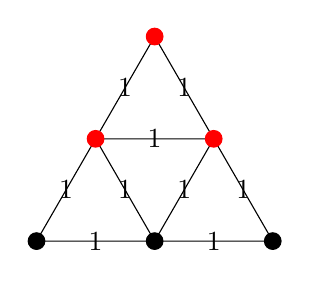
\begin{tikzpicture}[scale=3]
          \draw (0,0) -- node{1} (.5,0) -- node{1} (1,0) -- node{1} (.75,.433) -- node{1} (0.5,0.866) -- node{1} (.25,.433) -- node{1} (0,0);
          \draw (0.5,0) -- node{1} (0.25,0.433) -- node{1} (0.75,0.433) -- node{1} (0.5,0);
          
          \filldraw [black] (0,0) circle (1pt) ;
          \filldraw [black] (1,0) circle (1pt);
          \filldraw [red] (0.5,0.866) circle (1pt);
          \filldraw [black] (0.5,0) circle (1pt);
          \filldraw [red] (0.25,0.433) circle (1pt);
          \filldraw [red] (0.75,0.433) circle (1pt);
        \end{tikzpicture}\\
        \centering
      \end{figure}
      
    \end{column}
    \begin{column}{.3\textwidth}
      \begin{figure}
        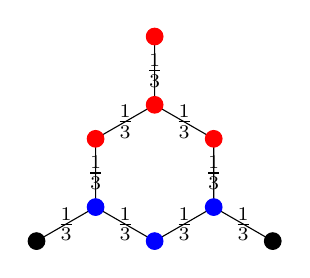
\begin{tikzpicture}[scale=3]
          \draw (0,0) -- node{$\frac{1}{3}$} (.25,.144) -- node{$\frac{1}{3}$} (.25,.433) -- node{$\frac{1}{3}$} (.5,.577);
          \draw (.5,.866) -- node{$\frac{1}{3}$} (.5,.577) -- node{$\frac{1}{3}$} (.75,.433) -- node{$\frac{1}{3}$} (.75,.144);
          \draw (.25,.144) -- node{$\frac{1}{3}$} (.5,.0) -- node{$\frac{1}{3}$} (.75,.144) -- node{$\frac{1}{3}$} (1.0,.0);

          \filldraw [black] (0,0) circle (1pt);
          \filldraw [black] (1,0) circle (1pt);
          \filldraw [red] (0.5,0.866) circle (1pt);
          \filldraw [blue] (0.5,0) circle (1pt);
          \filldraw [red] (0.25,0.433) circle (1pt);
          \filldraw [red] (0.75,0.433) circle (1pt);
          \filldraw [blue] (0.25,0.144) circle (1pt);
          \filldraw [blue] (0.75,0.144) circle (1pt);
          \filldraw [red] (0.5,0.577) circle (1pt);
        \end{tikzpicture}\\
        \centering
        % Resistors in series
        
      \end{figure}
      
    \end{column}


    
    \begin{column}{.3\textwidth}
      \begin{figure}
        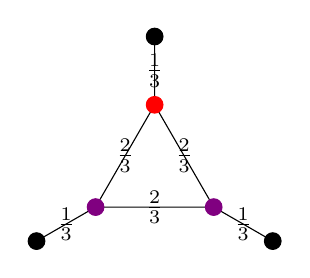
\begin{tikzpicture}[scale=3]
          \draw (0,0) -- node{$\frac{1}{3}$} (.25,.144) -- node{$\frac{2}{3}$} (.5,.577);
          \draw (.5,.866) -- node{$\frac{1}{3}$} (.5,.577) -- node{$\frac{2}{3}$} (.75,.144);
          \draw (.25,.144) -- node{$\frac{2}{3}$} (.75,.144) -- node{$\frac{1}{3}$} (1.0,.0);
          
          \filldraw [black] (0,0) circle (1pt);
          \filldraw [black] (1,0) circle (1pt);
          \filldraw [black] (0.5,0.866) circle (1pt);
          \filldraw [blue!50!red] (0.25,0.144) circle (1pt);
          \filldraw [blue!50!red] (0.75,0.144) circle (1pt);
          \filldraw [red] (0.5,0.577) circle (1pt);
         
        \end{tikzpicture}\\
        \centering
        % \dwt
      \end{figure}
      
    \end{column}
    
  \end{columns}


  
  \begin{columns}
    \begin{column}{.3\textwidth}
      \begin{figure}
        \centering
        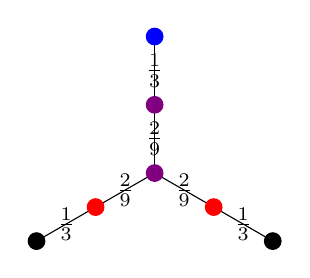
\begin{tikzpicture}[scale=3]
          \draw (0,0) -- node{$\frac{1}{3}$} (.25,.144) -- node{$\frac{2}{9}$} (.5,.288);
          \draw (.5,.866) -- node{$\frac{1}{3}$} (.5,.577) -- node{$\frac{2}{9}$} (.5,.288);
          \draw (.5,.288) --node{$\frac{2}{9}$} (.75,.144) -- node{$\frac{1}{3}$} (1.0,.0);         

          \filldraw [black] (0,0) circle (1pt);
          \filldraw [black] (1,0) circle (1pt);
          \filldraw [blue] (0.5,0.866) circle (1pt);

          \filldraw [red] (0.25,0.144) circle (1pt);
          \filldraw [red] (0.75,0.144) circle (1pt);
          \filldraw [red!50!blue] (0.5,0.577) circle (1pt);
          \filldraw [red!50!blue] (.5,.288) circle (1pt);
        \end{tikzpicture}\\
        % Resistors in series
      \end{figure}
      
    \end{column}

    \begin{column}{.3\textwidth}
      \begin{figure}
        \centering
        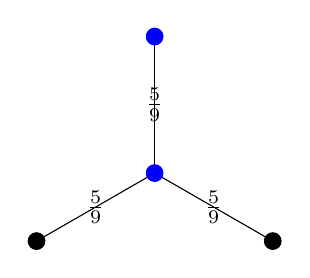
\begin{tikzpicture}[scale=3]         
          \draw (0,0) -- node{$\frac{5}{9}$} (.5,.288);
          \draw (.5,.866)-- node{$\frac{5}{9}$} (.5,.288);
          \draw (.5,.288) -- node{$\frac{5}{9}$} (1.0,.0);

          \filldraw [black] (0,0) circle (1pt);
          \filldraw [black] (1,0) circle (1pt);
          \filldraw [blue] (0.5,0.866) circle (1pt);

          \filldraw [blue] (.5,.288) circle (1pt);
        \end{tikzpicture}\\
        % \dwt
      \end{figure}
      
    \end{column}

    \begin{column}{.3\textwidth}
      \begin{figure}
        \centering
        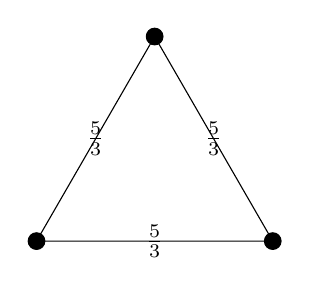
\begin{tikzpicture}[scale=3]
          \filldraw [black] (0,0) circle (1pt);
          \filldraw [black] (1,0) circle (1pt);
          \filldraw [black] (0.5,0.866) circle (1pt);
          
          \draw (.0,.0) -- node{$\frac{5}{3}$} (.5,.866) -- node{$\frac{5}{3}$} (1.0,.0) -- node{$\frac{5}{3}$} (.0,.0);
        \end{tikzpicture}\\
      \end{figure}
      
    \end{column}
  \end{columns}
    \medskip  
    Hence renormalization factor $r=\frac{3}{5}$.

   
\end{frame}




% ============================================================
% §1.6 Effective Resistance Metric
% ============================================================

\section{Effective Resistance Metric}

\begin{frame}[allowframebreaks=.95]{Effective Resistance}
    
    Given a nework, we define the effective resistance between any two points as the resistance between them when restricting to these two points:
    
    \begin{definition}[Effective Resistance]
    Let $x,y \in V$.
        \begin{align*}
            R(x,y)^{-1} := \min \left\{ \E(u) \,\middle\vert\, u(x)=0 \text{ and } u(y)=1 \right\} 
        \end{align*}
    \end{definition}
    \bigskip

    \textbf{Claim.} Equivalent: Minimum value for $R$ such that
    \begin{align*}
        \abs{u(x) - u(y)}^{2} &\leq R\, \E(u) && \text{for all } u \in \dom{\E}.
    \end{align*}
    \bigskip
    \newpage
    
    \textbf{Proof.} Let $u\in \dom{\E}$ such that $u(x)=0$ and $u(y)=1$ and $u$ minimizes $\E(u)$. Thus
    \begin{align*}
        1 = \abs{u(x) - u(y)}^{2} \leq R\, \E(u) = \frac{R}{R(x,y)}
    \end{align*}
    yields $R(x,y) \leq R$.

    For arbitrary $u \in \dom{\E}$ with $u(x) \neq u(y)$ denote $v := \frac{u - u(x)}{u(y)-u(x)}$.
    \note{If u such that u(x) \neq u(y) does not exist the claim is trivial.}
    Then $v(x)=0$ and $v(y)=1$ and
    \begin{align*}
        R(x,y)^{-1} \leq \E(v) = \frac{\E(u)}{\abs{u(x)-u(y)}^{2}}
    \end{align*}
    yields $\abs{u(x)-u(y)}^{2} \leq R(x,y)\,\E(u)$ and therefore $R \leq R(x,y)$.
\end{frame}

\begin{frame}{Effective Resistance on Unit Interval}
  Same as Eucledian distance:
  \begin{itemize}
  \item Function $u$ achieving minimum in definition of eff. resistance is
    harmonic in the complement of $x,y$.  Thus $u$ is the linear
    extension:
    \begin{align*}
      u(t) &=
      \begin{cases}
        0 & t \in [0,x) ,\\
        \frac{t-x}{y-x} & t \in [x,y) ,\\
        1 & t \in [y,1]
      \end{cases} && (\text{assume } x<y).
    \end{align*}
  \item Hence
    \begin{align*}
      \E(u)
      = \int_{0}^{1} \abs{u^{\prime}(t)}^{2} \, \mathrm{d}t
      =\int_{x}^{y}  \frac{1}{(y-x)^{2}} \, \mathrm{d}t
      = \frac{1}{y-x}
    \end{align*}
  \item We obtain
    \begin{align*}
      R(x,y) = \abs{y-x}.
    \end{align*}
  \end{itemize}
  
\end{frame}

\begin{frame}{Effective Resistance is Metric}
    \begin{theorem}[Tower Property]
        Suppose $V^{\prime\prime} \subseteq V^{\prime} \subseteq V$. Given a network on $V$, the restriction to $V^{\prime\prime}$ is equal to the restriction $V^{\prime\prime}$ of the restrction to $V^{\prime}$.
    \end{theorem}
    \bigskip
    
    \textbf{Claim.} Effective resistance fullfills triangle inequality.
    \bigskip

    \textbf{Proof.} Only need to consider $\Delta$-shaped networks. Combine rules for resistors in series and in parallel:

    \begin{columns}[c]
        \begin{column}{.7\textwidth}
            \begin{align*}
                R(x,y) &= \frac{1}{\frac{1}{R_{xy}} + \frac{1}{R_{yz} + R_{zx}}}
                = \frac{R_{xy}\,(R_{yz} + R_{zx})}{R_{xy} + R_{yz} + R_{zx}}
            \end{align*}
        \end{column}

        \begin{column}{.2\textwidth}
            \centering
            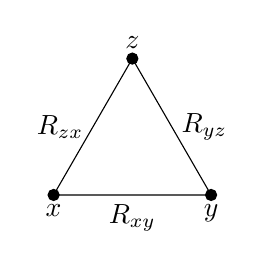
\begin{tikzpicture}[scale=2]
                \filldraw[black] (0,0) circle (1pt) node[below]{$x$};
                \filldraw[black] (1,0) circle (1pt) node[below]{$y$};
                \filldraw[black] (.5,.866) circle (1pt) node[above]{$z$};

               \draw (0,0)
                -- node[below]{$R_{xy}$} (1,0)
                -- node[right]{$R_{yz}$} (.5,.866)
                -- node[left]{$R_{zx}$} (0,0);
            \end{tikzpicture}
        \end{column}
    \end{columns}
    
    Short computation shows
    \begin{align*}
        R(x,y) + R(y,z) = R(z,x) + \frac{2\, R_{xy}\, R_{yz}}{R_{xy} + R_{yz} + R_{zx}} \geq R(z,x).
    \end{align*}   
\end{frame}

\begin{frame}[allowframebreaks]{Effective Resistance on SG}
    \note{Computing effective resistance is complicated. We can give estimates.}

    %\textbf{Aim:} Estimates for $R$.

    \begin{itemize}
        \item Consider neighboring vertices $x,y \in V_{m}$.

        \item Chose $u=\psi^{m}_{y}$ as piecewise harmonic spline, i.e. $\psi^{m}_{y}(z) = \delta_{yz}$ for all $z\in V_{m}$. Then
        \begin{align*}
            \E(u) = \E_{m}(u) = r^{-m}\, E_{m}(u) = r^{-m}\, \sum_{x\sim_m y} \abs{u(x) - u(y)}^{2} \leq 4\,r^{-m}.
        \end{align*}
        \note{Node $y$ has at most 4 neighbors.}
        Hence $R(x,y)^{-1} \leq \E(u) \leq 4\,r^{-m}$.
        
        \item $u(x)=0$ and $u(y)=1$ implies
        \begin{align*}
        \E(u) \geq \E_{m}(u) = r^{-m}\, E_{m}(u) \geq r^{-m}\, \abs{u(x) - u(y)}^{2} = r^{-m}.
        \end{align*}
        \item Conclude
        \begin{align*}
            r^{-m}\leq R(x,y)^{-1} \leq 4\, r^{-m}.
        \end{align*}
        \note{Remember definition of $R(x,y)$.}
        Thus $R(x,y) \sim r^{m}$.
    \end{itemize}
    \newpage
    
    Expansion to other points is possible:
    \begin{theorem}[Estimates for R]
        There exist $C_{1}, C_{2} > 0$ such that
        \begin{enumerate}[(a)]
            \item if $x,y$ are in the same or adjecent $m$-cells
            \begin{align*}
                R(x,y) \leq C_{1}\,r^{m}.
            \end{align*}
            \item if $x,y$ are \emph{not} in the same or adjecent $m$-cells
            \begin{align*}
                R(x,y) \geq C_{2}\,r^{m}.
            \end{align*}
        \end{enumerate}
    \end{theorem}
    \newpage

    \note{$x,y$ are neighbors again.}
    Consider SG on equilateral triangle with edge length 1 and neighboring vertices $x,y \in V_{m}$:
    \begin{itemize}
        \item $\abs{x-y}=2^{-m} = \exp(m\, \log{1/2}) \quad\implies\quad m = \frac{\log\abs{x-y}}{\log{1/2}}$.
        \item Obtain
        \begin{align*}
            r^{m} = \exp(m\, \log{r})
            = \exp\left( \frac{\log\abs{x-y}}{\log{1/2}} \, \log{r} \right)
            =: \abs{x-y}^{\beta}
        \end{align*}
        with
        \begin{align*}
            \beta = \frac{\log{r}}{\log{1/2}}
            = \frac{-\log{1/r}}{-\log{2}}
            = \frac{\log{5/3}}{\log{2}}
        \end{align*}
        \note{$r = \frac{3}{5}$.}
        \item Thus
        \begin{align*}
            R(x,y) &\sim \abs{x-y}^{\beta} && \text{with } \beta < 1.
        \end{align*}
        \item Effective resistance and Euclidian metric are topologically equivalent but they are not equivalent metrics.
        \note{Since $\beta < 1$ (small) distances in resistance metric are much larger than in Euclidean metric.}
    \end{itemize}
\end{frame}


%%% Local Variables:
%%% mode: latex
%%% TeX-master: "./main"
%%% ispell-local-dictionary: "american"
%%% End:
\end{document}